\section{The electrical field in between two charged parallel plates}
The electrical field in between two parallel plates will be \underline{uniform}\\

\begin{center}
\tikzset{every picture/.style={line width=0.75pt}} %set default line width to 0.75pt        

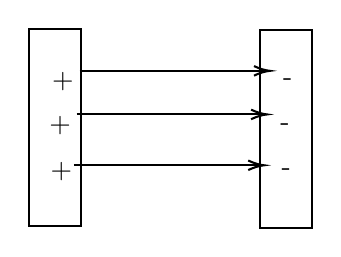
\begin{tikzpicture}[x=0.75pt,y=0.75pt,yscale=-0.7,xscale=0.7]
%uncomment if require: \path (0,300); %set diagram left start at 0, and has height of 300

%Shape: Rectangle [id:dp7601312066200475] 
\draw   (203,86) -- (239,86) -- (239,222) -- (203,222) -- cycle ;
%Shape: Rectangle [id:dp6408299179466447] 
\draw   (362,87) -- (398,87) -- (398,223) -- (362,223) -- cycle ;
%Straight Lines [id:da25512227366676565] 
\draw    (238,115) -- (367,115) ;
\draw [shift={(369,115)}, rotate = 180] [color={rgb, 255:red, 0; green, 0; blue, 0 }  ][line width=0.75]    (10.93,-3.29) .. controls (6.95,-1.4) and (3.31,-0.3) .. (0,0) .. controls (3.31,0.3) and (6.95,1.4) .. (10.93,3.29)   ;
%Straight Lines [id:da24494691864609286] 
\draw    (236,145) -- (365,145) ;
\draw [shift={(367,145)}, rotate = 180] [color={rgb, 255:red, 0; green, 0; blue, 0 }  ][line width=0.75]    (10.93,-3.29) .. controls (6.95,-1.4) and (3.31,-0.3) .. (0,0) .. controls (3.31,0.3) and (6.95,1.4) .. (10.93,3.29)   ;
%Straight Lines [id:da8099978455991589] 
\draw    (234,180) -- (363,180) ;
\draw [shift={(365,180)}, rotate = 180] [color={rgb, 255:red, 0; green, 0; blue, 0 }  ][line width=0.75]    (10.93,-3.29) .. controls (6.95,-1.4) and (3.31,-0.3) .. (0,0) .. controls (3.31,0.3) and (6.95,1.4) .. (10.93,3.29)   ;

% Text Node
\draw (215,144) node [anchor=north west][inner sep=0.75pt]   [align=left] {+};
% Text Node
\draw (216,176) node [anchor=north west][inner sep=0.75pt]   [align=left] {+};
% Text Node
\draw (217,114) node [anchor=north west][inner sep=0.75pt]   [align=left] {+};
% Text Node
\draw (374,146) node [anchor=north west][inner sep=0.75pt]   [align=left] {\mbox{-}};
% Text Node
\draw (375,177) node [anchor=north west][inner sep=0.75pt]   [align=left] {\mbox{-}};
% Text Node
\draw (376,115) node [anchor=north west][inner sep=0.75pt]   [align=left] {\mbox{-}};
\end{tikzpicture}
\end {center}

\subsubsection{Derive of $\mathcal{E} = \frac{\Delta V}{d}$}
Consider a negative charge of q that starts at the positive plate and is pushed at a constant velocity toward the negative plate (by some force)

\begin{center}
    \tikzset{every picture/.style={line width=0.75pt}} %set default line width to 0.75pt        

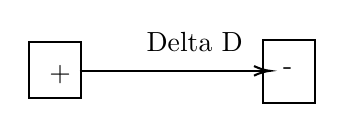
\begin{tikzpicture}[x=0.75pt,y=0.75pt,yscale=-0.7,xscale=0.7]
%uncomment if require: \path (0,300); %set diagram left start at 0, and has height of 300

%Shape: Rectangle [id:dp7601312066200475] 
\draw   (203,95) -- (239,95) -- (239,134) -- (203,134) -- cycle ;
%Shape: Rectangle [id:dp6408299179466447] 
\draw   (364,94) -- (400,94) -- (400,137) -- (364,137) -- cycle ;
%Straight Lines [id:da25512227366676565] 
\draw    (238,115) -- (367,115) ;
\draw [shift={(369,115)}, rotate = 180] [color={rgb, 255:red, 0; green, 0; blue, 0 }  ][line width=0.75]    (10.93,-3.29) .. controls (6.95,-1.4) and (3.31,-0.3) .. (0,0) .. controls (3.31,0.3) and (6.95,1.4) .. (10.93,3.29)   ;

% Text Node
\draw (215,109) node [anchor=north west][inner sep=0.75pt]   [align=left] {+};
% Text Node
\draw (376,107) node [anchor=north west][inner sep=0.75pt]   [align=left] {\mbox{-}};
% Text Node
\draw (282,86) node [anchor=north west][inner sep=0.75pt]   [align=left] {Delta D};


\end{tikzpicture}

\end{center}

\begin{center}
    \tikzset{every picture/.style={line width=0.75pt}} %set default line width to 0.75pt        

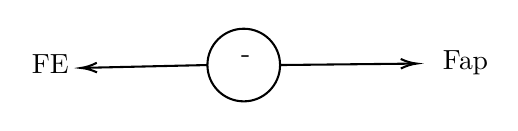
\begin{tikzpicture}[x=0.75pt,y=0.75pt,yscale=-0.7,xscale=0.7]
%uncomment if require: \path (0,300); %set diagram left start at 0, and has height of 300

%Shape: Circle [id:dp1650808345927549] 
\draw   (299,144) .. controls (299,130.19) and (310.19,119) .. (324,119) .. controls (337.81,119) and (349,130.19) .. (349,144) .. controls (349,157.81) and (337.81,169) .. (324,169) .. controls (310.19,169) and (299,157.81) .. (299,144) -- cycle ;
%Straight Lines [id:da03320137421401437] 
\draw    (349,144) -- (441,143.02) ;
\draw [shift={(443,143)}, rotate = 179.39] [color={rgb, 255:red, 0; green, 0; blue, 0 }  ][line width=0.75]    (10.93,-3.29) .. controls (6.95,-1.4) and (3.31,-0.3) .. (0,0) .. controls (3.31,0.3) and (6.95,1.4) .. (10.93,3.29)   ;
%Straight Lines [id:da771192465204896] 
\draw    (299,144) -- (214,145.95) ;
\draw [shift={(212,146)}, rotate = 358.68] [color={rgb, 255:red, 0; green, 0; blue, 0 }  ][line width=0.75]    (10.93,-3.29) .. controls (6.95,-1.4) and (3.31,-0.3) .. (0,0) .. controls (3.31,0.3) and (6.95,1.4) .. (10.93,3.29)   ;

% Text Node
\draw (320,132) node [anchor=north west][inner sep=0.75pt]   [align=left] {\mbox{-}};
% Text Node
\draw (459,132) node [anchor=north west][inner sep=0.75pt]   [align=left] {Fap};
% Text Node
\draw (176,135) node [anchor=north west][inner sep=0.75pt]   [align=left] {FE};

\end{tikzpicture}
\end{center}

\begin{lemma}
    $ W_{F_{ap}} = \mathcal{E}qd $
\end{lemma}

To start of, let's solve for $F_{ap}$
\begin{gather}
    \sum \vec{F} = 0 \nonumber \\
    F_{ap} - F_{E} = 0 \nonumber \\
    F_{ap} = F_{E} \nonumber \\
    F_{ap} = \mathcal{E}q\label{eq6.1}
\end{gather}

Next, let's solve for $W_{F_{ap}}$
\begin{gather}
    W_{F_{ap}} = F_{ap} \times \Delta d \times \cos\theta \nonumber
\end{gather}

Sub \ref{eq6.1} in to this equation:
\begin{gather}
    W_{F_{ap}} = (\mathcal{E}q) \Delta d \times 1 \nonumber \\
    W_{F_{ap}} = \mathcal{E}qd 
\end{gather}

The applied force has transferred kinetic energy into q, but q's kinetic energy hasn't changed. The electrical force is doing negative work on q, transferring
 the kinetic energy that the applied force gave to q into electrical potential energy

 \begin{theorem}
    $\mathcal{E} = \frac{\left | \Delta V \right |}{d}$ (This is only work for parallel plate question) You need to think about the direction conceptually!
 \end{theorem}

 \begin{gather*}
    \Delta E_E = W_{F_{ap}}\\
    \Delta E_E = \mathcal{E}qd\\
    q \Delta V = \mathcal{E}qd\\
    \Delta V = \mathcal{E}d\\
    \mathcal{E} = \frac{\Delta V}{d}
 \end{gather*}

 \noindent\hrulefill

When we deal with two charged parallel plate, we can say:
\begin{gather*}
    \Delta E_E = -\Delta E_k
\end{gather*}

When we release the electron, the energy will transfer from Electrical Potential Energy into Kinetic Energy. Kinetic energy increases and Electrical Potential Energy decreases. \\

We can rearrange this equation:
\begin{equation*}
    \Delta E_E + \Delta E_k = 0
\end{equation*}

\noindent\hrulefill

The formula for the electric potential difference for parallel plates is the same as for point charges:
\begin{equation}
    \Delta E_E = q\Delta V
\end{equation}

What if the charge between the plates doesn't travel as the way from one plate to another plate?
\begin{center}
    \tikzset{every picture/.style={line width=0.75pt}} %set default line width to 0.75pt        

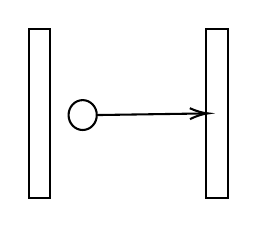
\begin{tikzpicture}[x=0.75pt,y=0.75pt,yscale=-0.8,xscale=0.8]
%uncomment if require: \path (0,300); %set diagram left start at 0, and has height of 300

%Shape: Rectangle [id:dp1602417857346311] 
\draw   (157,104) -- (170,104) -- (170,206) -- (157,206) -- cycle ;
%Shape: Rectangle [id:dp5155431267253283] 
\draw   (264,104) -- (277,104) -- (277,206) -- (264,206) -- cycle ;
%Flowchart: Connector [id:dp8574114031756601] 
\draw   (181,156) .. controls (181,151.03) and (184.81,147) .. (189.5,147) .. controls (194.19,147) and (198,151.03) .. (198,156) .. controls (198,160.97) and (194.19,165) .. (189.5,165) .. controls (184.81,165) and (181,160.97) .. (181,156) -- cycle ;
%Straight Lines [id:da11011233337200033] 
\draw    (198,156) -- (263,155.03) ;
\draw [shift={(265,155)}, rotate = 179.14] [color={rgb, 255:red, 0; green, 0; blue, 0 }  ][line width=0.75]    (10.93,-3.29) .. controls (6.95,-1.4) and (3.31,-0.3) .. (0,0) .. controls (3.31,0.3) and (6.95,1.4) .. (10.93,3.29)   ;

\end{tikzpicture}
\end{center}

\begin{equation}
    \Delta E_E = q\Delta V (\frac{x}{d})
\end{equation}
\begin{center}
    $d$ equals to the total gap between these two parallel plates\\
    $x$ equals to the distance that the charged particle will move
\end{center}